\documentclass[12pt]{article}
\usepackage[utf8]{inputenc}
\usepackage{amsmath}
\usepackage{amsfonts}
\usepackage{amssymb}
\usepackage{graphicx}
\usepackage{booktabs}
\usepackage{geometry}
\geometry{margin=1in}
\usepackage{float}
\usepackage{booktabs}  % For \toprule, \midrule, \bottomrule
\usepackage{array}     % For p{width} column type (paragraph columns)
\usepackage{subcaption}




\usepackage{amsmath}   % for \underset, aligned math
\usepackage{amssymb}   % for \mathbb{1} and \mathbb{R}
\usepackage{bbm}       % alternatively, for \mathbbm{1} (bolder indicator)
\DeclareMathOperator*{\argmin}{arg\,min}


\newcommand{\E}{\mathbb{E}}
\newcommand{\I}{\mathcal{I}}
\usepackage{setspace}
\onehalfspacing

\bibliographystyle{apacite}
\usepackage[nosectionbib,numberedbib]{apacite}

\usepackage{natbib}
%\bibliographystyle{abbrvnat}
\setcitestyle{authoryear,open={(},close={)}}
\usepackage{breakcites}

\usepackage[affil-it]{authblk}

\usepackage{xcolor}
\usepackage{hyperref}
\hypersetup{
    colorlinks  = true,
    citecolor   = darkgray,      % color for citations
    linkcolor   = blue,      % color for internal links
    urlcolor    = blue       % color for URLs
}

\title{Term paper proposal: Growth-at-Risk}
\author{Jes\'us L\'opez-P\'erez\thanks{e-mail: \texttt{jlopezperez@gradcenter.cuny.edu}, Department of Economics, The Graduate Center\\ The City University of New York}}


\affil{Spring 2026}

\date{April 10, 2026}

\begin{document}

\maketitle


\section{Introduction}
Central banks when making monetary policy must account for various risks including real economic factors and financial risks. When doing a balance of risks these institutions weigh both downside risks --production, unemployment-- and upside risks --inflation. In addition, financial risk are usually associated with high volatility, that can be seen as an endogenous response to the business cycle or as an exogenous impulse to it \citep{ludvigson2021uncertainty}. 

The problem for the forecaster is then extended from the usual GDP growth point estimate to the broader task of estimating lower, middle and higher quantiles. These additional estimates can be later used for assessing the conditional mean of GDP growth on increased volatility of economic and financial conditions. For instance, the Survey of Professional Forecasters elicit not only point estimates, but also probabilities of point estimates for GDP growth, unemployment rate and inflation, see figure ~\ref{fig:spf_distributions_2026}.

The question at hand is thus:\textit{ what is the worst GDP outcome what we should expect with given probability?.} This has been tackled in the relevant study by \cite{adrian2019vulnerable}. The authors develop a framework --Growth-at-Risk (GaR)-- that allow to obtain the empirical quantile distribution --estimated conditional distribution of GDP-- based on preliminary lower, middle and upper quantiles. 


In this research I focus on the estimation of the empirial quantile distribution of GDP growth for the Mexican economy, see figure ~\ref{fig:gdp_growth}. The question is relevant because, unlike the US FOMC, the Mexican central bank does not have the dual mandate of keeping low inflation and achieving potential GDP growth. Banco de Mexico (Banxico) has only the low inflation mandate, thus its assessment of risks is not the same as in the US economy.


\section{Model (sketch)}
The quantile estimation, following \cite{adrian2019vulnerable} is given by: 

\begin{equation}
    \hat{\beta}_{\tau} = \underset{\beta_{\tau} \in \mathbbm{R}^{k}}{\argmin}
    \sum_{t=1}^{T-h} \left(
    \tau \cdot \mathbbm{1}_{(y_{t+h} \geq x_t \beta)}
    \left| y_{t+h} - x_t \beta_{\tau} \right|
    +
    (1 - \tau) \cdot \mathbbm{1}_{(y_{t+h} < x_t \beta)}
    \left| y_{t+h} - x_t \beta_{\tau} \right|
    \right)
\end{equation}

I will also consider the methodologies to assess uncertainty in \cite{Ferrara2022HFmonitoring}, \cite{Adrian2022TermStructure} and  \cite{GonzalezRivera2024ExpectingUnexpected} 


\section{Data}
Figure \ref{fig:gdp_growth} shows the evolution of yearly Mexican economy growth from Mexico's  \cite{inegi_gdp_quarterly_2026}. 
\begin{figure}[h]
\centering
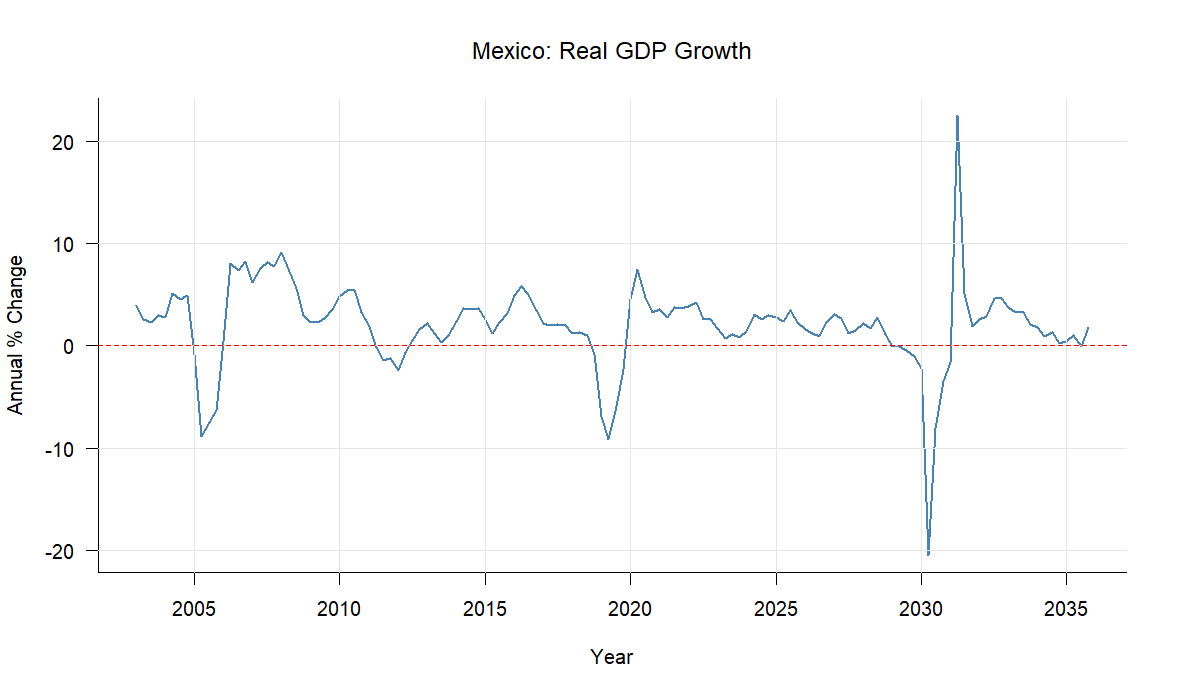
\includegraphics[scale=0.6]{gdp_growth.png}
\caption{Mexico's Real GDP Growth. Annual percentage change in real GDP. Source: INEGI.}\label{fig:gdp_growth}
\end{figure}


\bibliographystyle{apalike}
\bibliography{references}



\appendix

\centering
\begin{figure}[htbp]\label{spf-figure}
    \centering
    % Top row
    \begin{subfigure}[t]{0.48\textwidth}
        \centering
        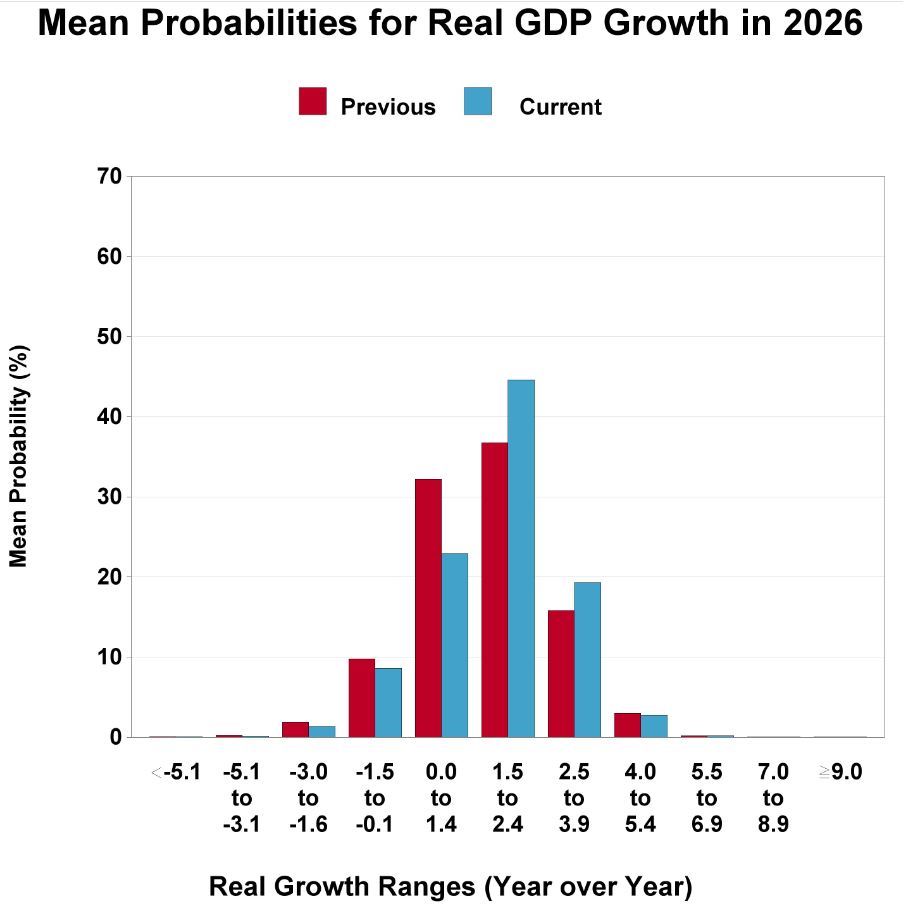
\includegraphics[width=\textwidth]{spf_prob_gdp_growth_2026}
    \end{subfigure}
    \hfill
    \begin{subfigure}[t]{0.48\textwidth}
        \centering
        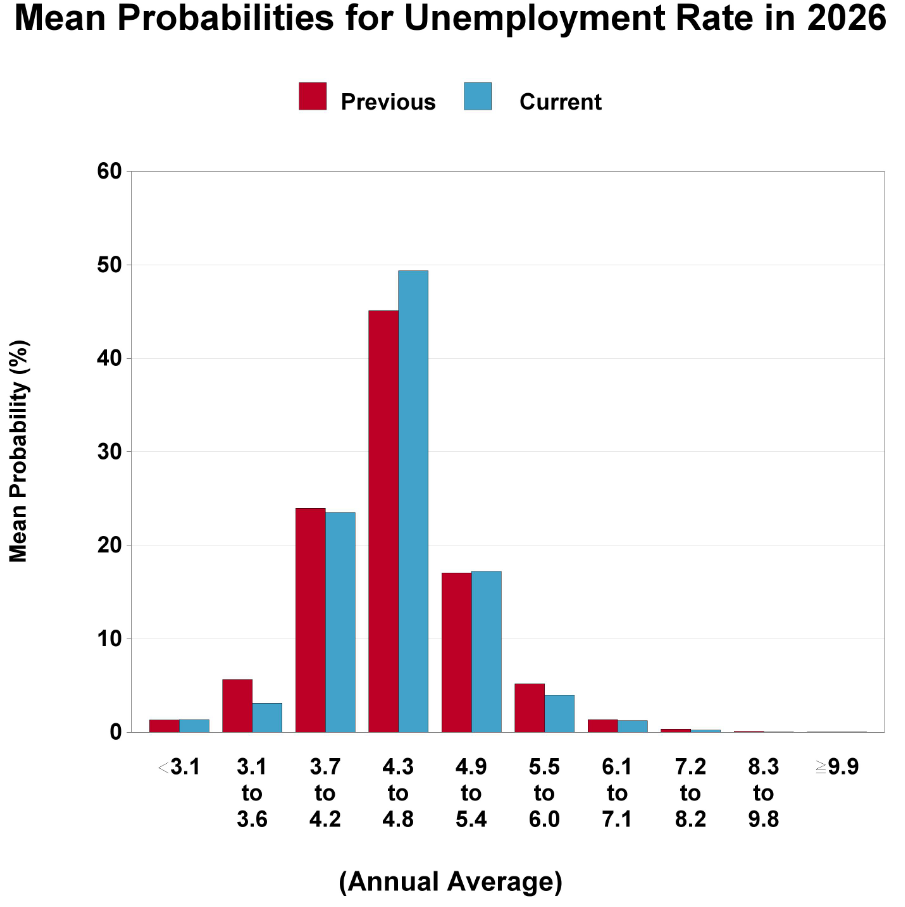
\includegraphics[width=\textwidth]{spf_prob_u_rate_2026}
    \end{subfigure}

    \vspace{0.5em}

    % Bottom row (centered)
    \begin{subfigure}[t]{0.48\textwidth}
        \centering
        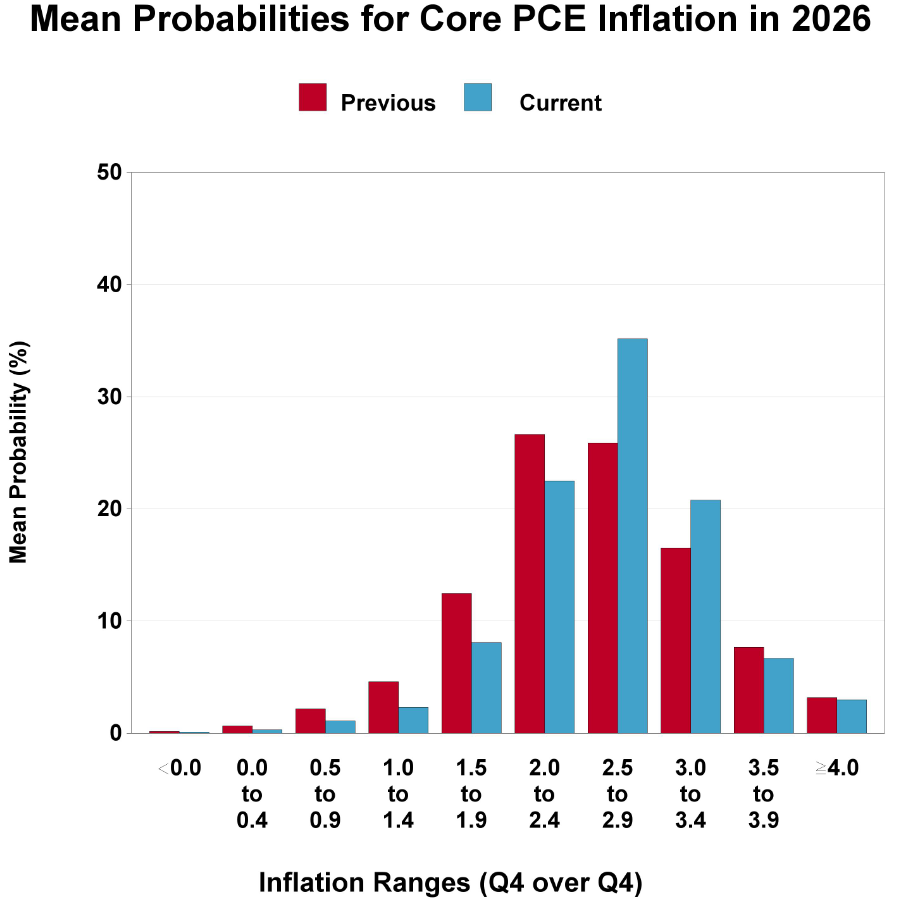
\includegraphics[width=\textwidth]{spf_prob_pce_inflation_2026}
    \end{subfigure}

    \caption{SPF Probability Distributions for 2026: GDP Growth (top left),
    Unemployment Rate (top right), and PCE Inflation (bottom). SPF, Nov 2025 \citep{philadelphiafed_spf_q4_2025}.}
    \label{fig:spf_distributions_2026}
\end{figure}






\end{document}